\chapter{Introduction}

\section{Unsolved questions in black hole astrophysics}

%- event horizons, strong gravity, black hole parameters, evolution of structure, 
%ref narayan 2013

%basics st 1
Black Holes (BHs) are both extreme and ubiquitous objects which are increasingly becoming seen as central to our understanding of the physical universe. The first inferences of their existence came from the observations of the highly energetic Active Galactic Nucleus (AGN) Cygnus~A as well as the rapid variability of quasars, both implying a massive and compact engine \citep[][and references therein]{Narayan_2013}. BHs are formed through the gravitational collapse of a stellar core during a supernovae explosion or from direct collapse from a primordial gas cloud and can grow in mass through accretion of nearby material and/or mergers with other black holes. The observed BH mass distribution is separated into two distinct mass classes, stellar and supermassive - the former with mass on the order $M \sim 10 M_\odot$ and the latter $M \sim 10^6 - 10^{10} M_\odot$ \citep{Falcke_2013}. Here we will focus on the class of supermassive black holes (SMBHs) for reasons provided shortly.


%observational traits and energy -reading needed
Accretion of gas onto the SMBH releases gravitational energy, which heats the relativistic gas disc  The dominant emission mechanism is synchrotron. The classical idea of an Active Galactic Nucleus (AGN) is a SMBH surrounded by an accretion disc ejecting a jet along it's polar axis. The jets can remain collimate over large cosmic distances. magnetic fields

 
%host galaxy interaction - reading needed
SMBHs form and reside (unless ejected) in the centres of all galaxies \citep{Kormendy_1995}. Observations of their surrounding galactic bulges show tight correlations between BH mass and the bulge luminosity and stellar velocity dispersion, suggesting coevolution or feedback processes. This can take the form of gas ejection or ionisation and associated heating of the surrounding medium. 


%this is the last line of the basics - oh yeah
The past half century has seen signficant advances in BH theory and observation, however key questions remain unsolved - until now perhaps.
However much of the work on black holes emission mechanisms and dynamics remain inconclusive as no observation has yet been able to resolve the AGN at it's core. 
%the need for direct, resolved observations o



%constraining event horizon scale physics + SgrA is best candidate #gravitational radius aas a quantity?
To constrain the physics near a black hole, the observation needs to be sensitive to scales comparable to the event horizon. For a non-spinning (Schwarschild) black hole, the event horizon is spherically symmetric with a radius, 
\begin{equation}
R_{\rm Sch} = 2 G M_{\rm BH} /c^2,
\end{equation}
where $M_{\rm BH}$ is the black hole mass, $G$ is the gravitational constant and $c$ is the speed of light. The angular size of such an event horizon in the far-field approximation is
\begin{align}
\theta_{\rm Sch} &= R_{\rm Sch} / d_{\rm src}\\
&\approx 0.02^{\prime \prime} \times 10^{-9} (M_{\rm BH}/M_\odot)({\rm kpc}/d_{\rm src}),
\end{align}
where $d_{\rm src}$ is the distance from observer to source. For Sgr~A$^\star$, optical/infrared monitoring of stars orbiting Sgr~A* \citep{Gillessen_2009} has yielded ${M_{\rm BH} = 4.30 \pm 0.36 \times 10^{6} M_\odot}$ and ${d_{\rm src}= 8.28 \pm 0.32}$~kpc which results in ${\theta_{\rm Sch} \approx 10\ \mu}$-arcsec. 

%Highlight several questions - not even sure if we want subsections?
% can also interchange the order

\subsection{Spin, accretion and jet launch}
% 
extracting the rotational energy from the black hole
fundamental plane of black hole activity - accretion rate and black hole mass seems to determine jet power however theory suggests that spin should power the jet
In addition to probing the spacetime around black holes, the EHT will also enable unprecedented observations of the inner accretion and jet physics, the exact mechanisms and contexts of which are highly debated. Radiatively Inefficient Accretion Flow \citep[(RIAF),][]{Narayan_1995,Yuan_2003} models offer a popular explanation for the $\sim 10^{-8} L_{\rm edd}$ of Sgr~A*, however horizon scale observations are still needed to robustly compare models. In this model the electron and proton temperatures decouple due to the low density of the gas. Most of the gravitational energy is converted into the viscous thermal energy of protons which radiate inefficiently compared to electrons. The protons are then either advected into the SMBH or ejected via outflows possibly in the form of winds or a low powered jet. In contrast, the powerful jet in M87 is thought to be powered by an accretion disc in the Magnetically Arrested Disc \citep[(MAD),][]{Narayan_2003} state, wherein accretion on the BH is suppressed by strong poloidal fields. Additional questions include determining whether Sgr~A* is disc or jet dominated; the location of the jet base in M87 is in relation to its event horizon; whether the event horizon actually exists; and the orderedness of magnetic fields in the inner accretion disc and jet.
(ISCO)
spins have been measured for stellar mass black holes

%Lensing and the photon ring  st 1
Fortunately, the innermost emission is gravitationally lensed by the SMBH, which causes it to appear magnified by several times its original size. In theory, the innermost orbit should be dominated by a ring of photons, the lensed image of which should feature a shadow-like (or `silhouette') feature \citep[e.g.][]{Johannsen_2010}. Fig.~\ref{fig:grmhd} shows an image ray-traced from a General Relativistic Magneto-Hydrodynamic simulation of the accretion disc around Sgr~A* \citep{Moscibrodzka_2014} The circular shadow is apparent in the centre of the image. The two primary targets Sgr~A$^\star$ and M87 are expected to have gravitationally-lensed photon rings with apparent angular diameters of $\theta_{\rm pr} \sim 50$ and $\sim 20-40\ \mu$-arcsec respectively \citep*{Broderick_2009,Falcke_2013}, and hence should be resolvable by the EHT. 

% Emission and optical depth 
There are other important reasons why this observation needs to be conducted near sub-millimetre frequencies. Firstly, the spectral energy distribution of Sgr~A$^\star$ peaks sharply in sub-millimetre, which for a self-absorbed synchrotron source  implies that the emission becomes optically thin and at these frequencies, that the emission arises from event horizon scales \citep{Serabyn_1997,Falcke_1998}. Hence observations at the sub-millimetre are sensitive to the innermost emission.
%ISM blurring st 1
The second reason is that blurring effects, induced by scattering in the Interstellar Medium (ISM) in the direction of the Galactic Centre \citep[e.g.][]{Fish_2014} fall as $\nu^{-2}$ and become subdominant to intrinsic structure in the sub-millimetre range.


%st 1
\begin{figure}
\begin{center}
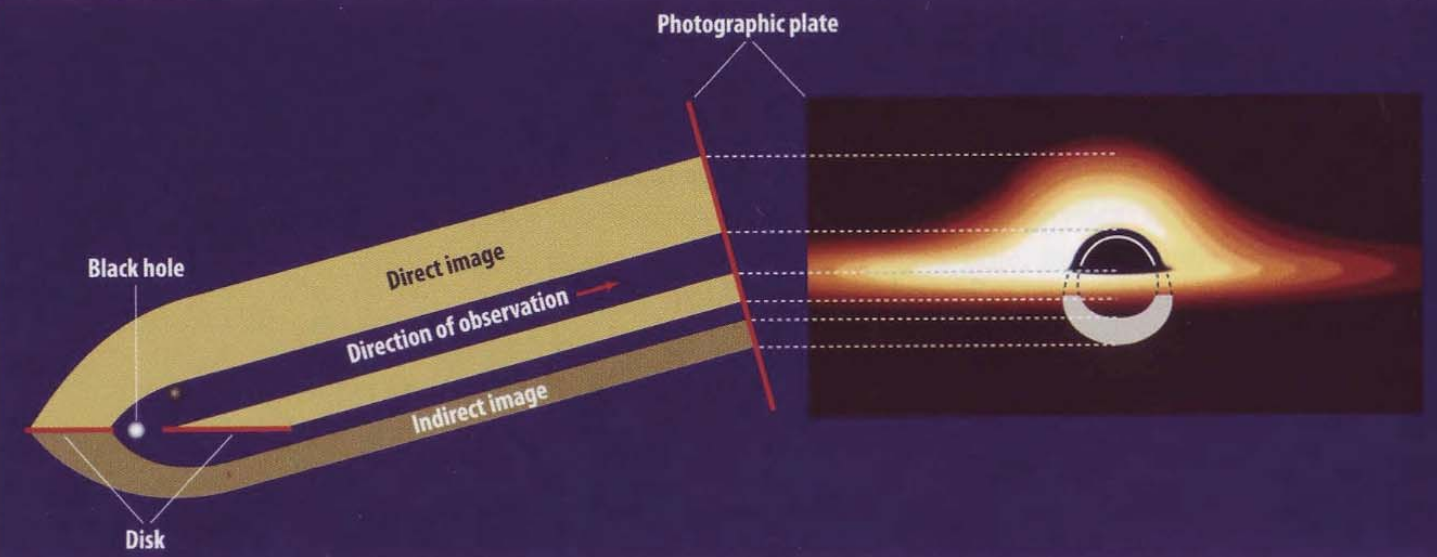
\includegraphics[width=\columnwidth]{Images/lensed_cartoon}
\caption{(Image credit : Shep Doeleman) Cartoon image (left) combined with the ray-tracing of a thin accretion disc surrounding a BH, first calculated by \citet{Luminet_1979}. The cartoon image shows that both the bottom and top of the back of the accretion disc is lensed by the black hole and becomes visible The dark area in the centre, known as the black hole shadow is the lensed image of the photon ring orbiting the BH. A measurement of it's precise shape is a test of general relativity in the strong field regime. Note that the left-right asymmetry in the image is due to doppler boosting, and that all sides of the accretion disk and photon ring are visible due to lensing. \label{fig:grmhd}%
}
\end{center}

\end{figure}



\subsection{Space-time in strong gravity}

%Probing strong gravity and black hole spacetime St 1
Gravity as described by General Relativity (GR) is consistent with all observational experiments thus far, however GR has conceptual weaknesses, especially as it is not compatible with the quantum description of reality. Various alternatives to GR have been theorised which do not assume a purely classical description of matter. To compare GR with the alternatives, we have to compare its predictions in the strong, non-linear field regime where the largest deviations from GR would occur if it were an approximate theory.


The spacetime within several $R_g$ around a SMBH provides this opportunity. The precise shape of the the photon ring around a SMBH is dependent on the spacetime which in turn is calculated within a theory of gravity \citep{Takahashi_2004}. The No-Hair theorem, which is based on GR, states that the spacetime should only be determined by the first two moments of the black hole, i.e. it's mass and spin. If the No-Hair theorem is invalid, the ring will deviate from a Schwarschild or Kerr profile. In the case of a non-zero quadrupole moment the ring will become either oblate or prolate \citep{Johannsen_2010}. This asymmetry is potentially measurable by EHT observations \citep{Broderick_2014}.

Is there an event horizon or a surface? - surface would radiate


\section{Cranking up the angular resolution}

%Increasing resolution -> motivation and difficulties
Throughout the history of astronomy, there have been celestial sources which appear point-like (unresolved) with the available instrumentation. To investigate the nature of these sources, ever more sophisticated instruments with higher resolution are developed. 

In principle, a diffraction-limited aperture can obtain an angular resolution of
\begin{equation}\label{eq:ang_res}
 \theta_{\rm res}\ \approx \ 1.22\ \lambda / D,
\end{equation}
where $D$ is the diameter of the aperture and $\lambda$ is the observing wavelength. However, dish apertures larger than a hundred metres are infeasible to construct while systematic errors, including scattering-induced blurring due to inhomogeneous density (radio) or temperature (optical) distributions in the Earth's atmosphere can lead to instrument being unable to reach the diffraction limit. To overcome these difficulties and improve $\theta_{\rm res}$, a variety of new technologies have been developed (see Fig~\ref{fig:spec_ang}), including space-based observatories which escape the limitations set by the Earth's atmosphere, interferometric arrays which eliminate the need to build extremely large apertures, as well as technology-enabled mitigation strategies like adaptive optics and water vapour radiometry which account for atmospheric turbulence in real time. 


%Very Long Baseline Interferometry -> the highest resolution
The observing technique which typically achieves the highest angular resolution is Very Long Baseline Interferometry (VLBI). Interferometry refers to the technique of measuring the electric field correlations (named `visibilities') between pairs of separated antennae. The visibilities are related to Fourier components on a section of approximately flat sky. Through an `adequate' sampling of the Fourier domain an approximate image of sky can be reconstructed using the inverse Fourier transform. With this method, the distance between the antennae ($\bm{b}$, referred to as the `baseline') effectively replaces $D$ in equation~\ref{eq:ang_res}, yielding a higher angular resolution than a single aperture. This technique is primarily used at radio frequencies while the electric field phase remains relatively stable. VLBI is essentially radio interferometry with antennae separated by large distances, typically $\gtrsim 100$~km, including the possibility for antennae in Earth's orbit. A key distinction from connected-element interferometery is that independent clocks are needed at each station to facilitate the post-observation correlation. VLBI has seen several noteworthy achievements since its inception in the late 1960's, including resolution of the extra-galactic, compact, highly-variable objects, now known as quasars into super-luminal core-jet systems \citep[e.g.][]{Whitney_1971}, and the mapping of maser motion around the Super-Massive Black Holes (SMBH) in the cores of nearby galaxies \citep[e.g.][]{Miyoshi_1995}.


%fig : angular resolution across spectrum
\begin{figure}
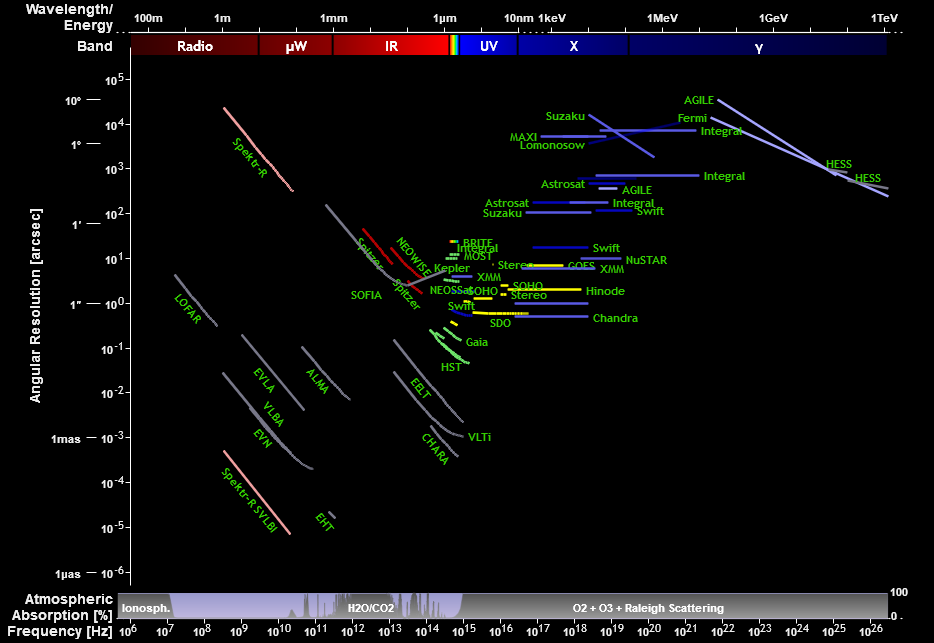
\includegraphics[width=\columnwidth]{Images/spec_ang}
\caption{(Image credit: Olaf Frohn\protect\footnote{http://armchairastronautics.blogspot.co.za/p/space-observatories.html}) An illustration of angular resolution vs. observing frequency across the entire observational spectrum, shown for a selection of observatories. The VLBI arrays : Spektr-R SVLBI (or RadioAstron) and the EHT clearly achieve the highest angular resolution of all due to their long baselines. At the bottom of the plot, there is a panel showing atmospheric/ionospheric absorption as a function of wavelength, and consequently all observatories in the zero transmission zones are space-based. \label{fig:spec_ang}
}
\end{figure}

As will be described in the next section, the ultra-high angular resolution provided by VLBI enables investigation into several key questions concerning black holes.



\section{The Event Horizon Telescope}
\subsection{Overview}

% EHT -> intro to the Array st 1
In the last few decades there has been a push to enhance VLBI capabilities at sub-millimetre wavelengths. One of the leading efforts in this regard is the Event Horizon Telescope consortium \citep[(EHT),][]{Doeleman_2010}, an international project whose primary objective is to spatially resolve the lensed photon rings nearby SMBHs with an angular resolution on the order of their event horizons. In contrast to competing high frequency VLBI observatories e.g. the Very Long Baseline Array (VLBA) which had coverage to 87~GHz (3~mm), the EHT is operating at 230~GHz (1.3~mm) and will potentially extend till 345~GHz (0.8~mm) in the future. See Fig.~\ref{fig:eht_globe} for an annotated map of the locations of the EHT array. As the EHT will have baseline lengths comparable to the diameter of the earth, $|b| \sim 10^4$~km and is operating at 1.3~mm, this yields $\theta_{\rm res} \sim 30\ \mu$-arcsec.

%st 1
\begin{figure}
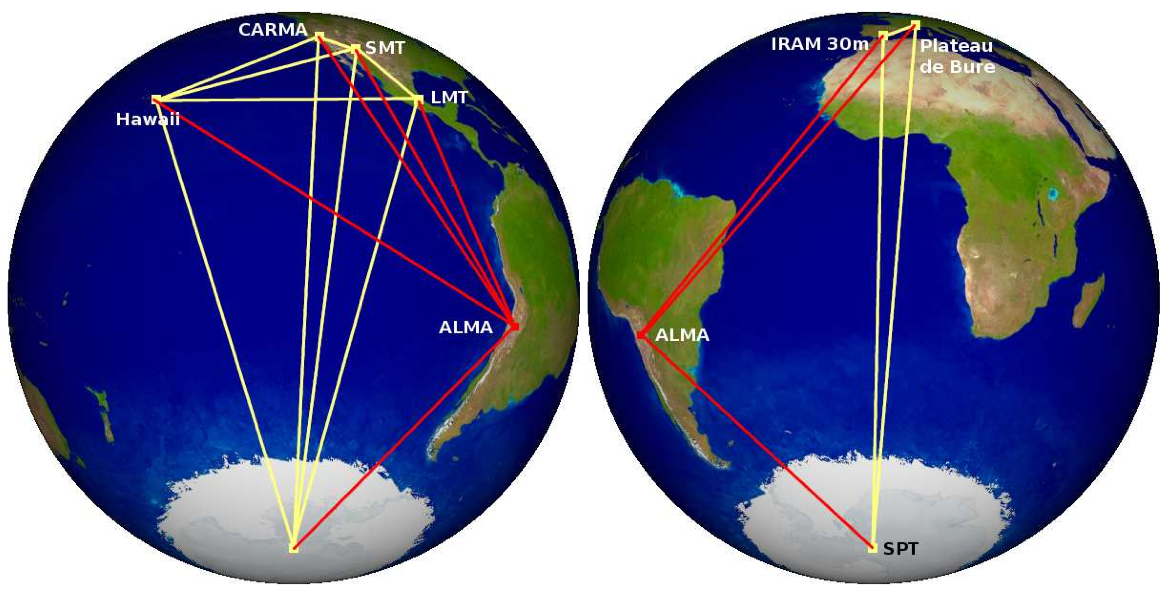
\includegraphics[width=0.8\columnwidth]{Images/eht_globe}
\caption{(Image credit: Remo Tilanus) The view of the Event Horizon Telescope (EHT) from Sgr~A*. This interferometric array uses Earth-diameter baselines, operating at $230-345$~GHz to attain an angular resolution of the order of ${\theta_{\rm res} \sim 10\ \mu}$-arcsec. Baselines to ALMA are shown in red, to highlight its order of magnitude higher sensitivity. Note that the CARMA station has recently been decommissioned, a telescope in Greenland is currently being constructed and there is ongoing investigation into a possible site on the African continent.\label{fig:eht_globe}%
}
\end{figure}



\subsubsection{Instrumentation and observational challenges}

%intro - newness of field and instrument st 1
The development of mm-VLBI instrumentation has been spurred by the formation of EHT as a project and the deepening of theory and simulation work over the past two decades. This is evidenced by the comparable observational results but starkly different interpretations of \citet{Krichbaum_1998} and \citet{Doeleman_2008}. A decade apart, both teams observed Sgr~A* with a mm-VLBI arrays consisting of three stations at similar frequency (215~GHz in 1998 and 230~GHz in 2008). Although the former was limited by calibration problems, the primary difference in analysis and interpretation was that the later result was linked explicitly to the innermost accretion physics in the event horizon region \citep[e.g.][]{Broderick_2011} i.e. the newly developed theoretical context contributed to the significance of the \citet{Doeleman_2008} result. However, to robustly interrogate this diverse body of theoretical work, an ultra-high precision instrument is needed. For example, to discern whether the No-Hair theorem is violated requires the fractional asymmetry of the shadow shape with respect to its angular size to be measured to a few percent \citep{Goddi_2016}. To achieve this level of precision, the development of the global mm-VLBI array will surely be faced with its fair share of obstacles.

%St : 1

%moving to higher freq st1
The move to higher frequencies is accompanied by requirements on the instrument including: increased data rates and stability of timing standards; as well as increased accuracy of dish surfaces and antenna pointing accuracy. Difficulties emerge also from the effects of the Earth's lower atmosphere where optical depth becomes significant and turbulence causes rapid fluctuations in the signal transmission time which causes decoherence in the visibilities. Even though the stations are in high altitude, desert locations, the atmospheric coherence times are still short, typically $\lesssim$10~s \citep{Doeleman_2009}. The extensive requirements on instruments and location push up the cost of mm-VLBI stations resulting in sparsely populated interferometric arrays which make for inadequate sampling of the Fourier domain. 




%More complicated effects
Aside from the considerations listed above, there are other important issues relevant to the target sources, the ISM and the calibration procedure. Firstly the line-of-sight to the Galactic Centre passes through an inhomogeneous turbulent electron plasma in the Interstellar Medium (ISM). This medium both blurs and introduces random, time-variable substructure into the source brightness distribution (see section~\ref{sec:ism_scat}). The scattering substructure adds substantial complications for data interpretation as its contribution is difficult to entangle from that of the intrinsic source substructure. The second issue is that the source itself is variable over minutes to hours (see section~\ref{sec:variability}). The fact that the source is variable over the course of a single observation epoch breaks a fundamental assumption in interferometry as the visibilities cannot be related to a single sky image. Additional complications arise due to the assumptions in self-calibration that the source is static, while in fact both the source and the ISM are time-variable. Traditional calibration is also difficult as the high frequency sky has a lower calibrator source density and calibrators are mostly resolved and possible variable too. 


% Effect of corruptions on Science extraction : parameter estimation and imaging, #HighAccuracy
These effects, among others, may place significant limitations on the sensitivity, image fidelity, and dynamic range that can be achieved with mm-VLBI.  Furthermore, unaccounted for systematic and/or non-Gaussian uncertainties could preclude robust, accurate Bayesian parameter estimation and model selection analyses of accretion flow \citep[e.g.][]{Broderick_2016} and gravitational physics \citep[e.g.][]{Broderick_2014, Psaltis_2016}, two of the EHT's many objectives. 


\section{A realistic mm-VLBI simulator}
%Pr : 1 : St : 1

%Why simulate: intro 
Given the significant observational challenges that the EHT faces, we have undertaken this project to build a mm-VLBI observation and signal corruption simulator. There are many benefits for using such a toolkit and indeed synthetic data simulation is common practice for major scientific experiments. A prominent example is the extensive gravitational wave template matching scheme for The Laser Interferometer Gravitational-Wave Observatory (LIGO) which operates in the presence of tidal loading, passing trains etc. In essence such a simulator would fill in the final component of the theoretical signal propagation chain, effectively taking astrophysical simulations of the source (e.g. accretion onto a SMBH) as an input and returning realistic synthetic interferometric data. This allows a more effective interplay between theory and observation, quantifying systematic effects and the measurement limits. The remainder of this section will briefly discuss several research questions relevant to an EHT synthetic data simulator and how we approach the software design in order to address these questions. 

%Specific use cases of simulations

%Testing calim through standard challenges 
A key use case for simulated data is the testing of calibration, parameter estimation and imaging algorithms and strategies. As the inputs to the simulator are known exactly, we are better able to explore sources of error which are difficult to disentangle from intrinsic source features when using only real data. A straightforward way to perform such a test is through the creation of a set of `standard challenge' dataset. Such datasets would be available to the entire community to input into their calibration and/or imaging routines. Following this, a detailed comparison between the different strategies in varying regimes (source, ISM, troposphere and instrumental) can be made. Importantly, a systematic investigation of a particular algorithm across many different datasets could provide insight into subtle or previously unknowns sources of error inherent in that routine.


%Optimising observations 
Simulated data can also assist in the optimisation of the experimental configuration. Financial constraints require the prioritisation of hardware upgrades e.g. increasing bandwidth, surface accuracy improvement, deployment of water vapour radiometers or additional receiver bands. Simulated data together with calibration and imaging pipelines can help to quantify the benefit of each improvement based on expected scientific return in units of precision of the scientific parameter of interest (e.g. shadow assymetry) rather than more generic terms (e.g. angular reso. This approach can even be extended to assess new candidate stations, especially as new geographic locations e.g. in Southern Africa are receiving increasing attention due to the potential long baselines to ALMA, SPT and European stations.


%other simulation efforts 
Recently, there has been an increase in the attention given to simulating EHT observations of Sgr~A*  and M87 \citep{Fish_2014,Lu_2014,Bouman_2015,Lu_2016,Chael_2016}. However, these are primarily focused on image reconstruction and assume either negligible or Gaussian distributed gain errors; perfect antenna pointing accuracy; and in most cases only Gaussian convolution to simulate ISM scattering. Clearly, as the EHT array is enhanced (and possibly expanded), so too must the interferometric simulations evolve to provide ever-more physical predictions on the confidence levels with which parameters can be extracted and hence exclude theoretical models of gravity and/or accretion flows.


%the Meqtrees+MS approach
Over the past decade, significant effort has been placed on advanced radio interferometric calibration and imaging algorithms for centimetre and metre-wave facilities in response to the large number of new arrays in construction or design phase (e.g. MeerKAT, ASKAP, SKA, LOFAR, HERA). A leading software package in this pursuit is \textsc{MeqTrees}\footnote{https://ska-sa.github.io/meqtrees/} \citep*{Noordam_2010}, which was developed to simulate, understand and address the calibration issues to be faced with the greatly enhanced sensitivity, instantaneous bandwidth, and field-of-view of such facilities. For example, \textsc{MeqTrees} is rooted in the Measurement Equation mathematical formalism \citep{Hamaker_1996}, which parameterizes the signal path into distinct $2 \times 2$ complex  matrices called Jones matrices. This formalism and applications thereof are laid out in \citep{Smirnov_2011a,Smirnov_2011b,Smirnov_2011c} and are arbitrarily generalized to model any (linear) effect, including undesired signal corruptions that often may have subtle yet systematic effects. \textsc{MeqTrees} has been applied to correct for direction dependent calibration errors to JVLA and WSRT observations, achieving record-breaking high dynamic range images \citep{Smirnov_2011c}. The effectiveness provided by the Measurement Equation formalism in radio interferometric calibration provides a strong motivation to explore its application to challenging goal of imaging a supermassive black hole silhouette with mm-VLBI. To construct this simulator we leverage off metre and cm-wavelength simulation and calibration successes and build a \textsc{MeqTrees}-based mm-VLBI-specific software package which we name, \textsc{MeqSilhouette}.  Use of \textsc{MeqTrees} and \textsc{measurement set} data format lends itself to investigating a range of different techniques that are used in other areas of interferometry (e.g. coh-Jones paper). While \textsc{MeqTrees} has not yet been used in the context of mm-wavelength observations, the framework is agnostic to higher frequency implementation as long as the Measurement Equation is appropriately constructed. 


\section{Outline}

This thesis is broadly divided into the following chapters and sections,
\begin{itemize}
 \item {\bf Chapter 2 : Theory} 
 \begin{description}
  \item [Section 2.1] introduces radio interferometry via the Measurement Equation formalism, followed by a brief discussions on a selection of topics relevant to mm-VLBI.
  \item [Section 2.2] is a review and investigation into the key signal corruptions to be implemented in our proposed mm-VLBI simulator.
 \end{description}

 \item {\bf Chapter 3 : Software Implementation}\\
 A description of the design and construction of the simulation software with emphasis on the software architechure and workflow.
 
 \item {\bf Chapter 4 : Results and Analysis}
 \begin{description}
  \item  [Section 4.1] showcases the basics of the simulator output through a series of canonical results.
  \item [Section 4.2] is a more sophisticated scenario involving calibration in ..
 \end{description}
  
  \item {\bf Chapter 5 : Conclusions and future work}\\
  We summarise the work and context of this thesis as well as make suggestions for future applications and improvements.
 
\end{itemize}
















